%%%%%%%%%%%%%%%%%%%%%%%%%%%%%%%%%%%%%%%%%%
%    File: ICTONmeetings.tex             %
%    Date: 2020                          %
%    inquiries: mikko.huttunen@tuni.fi   %
%                                        %
%    Home-made LaTeX template for ICTON  %
%%%%%%%%%%%%%%%%%%%%%%%%%%%%%%%%%%%%%%%%%%
 
\documentclass[letterpaper,10pt]{article} 
%% if A4 paper needed, change letterpaper to A4
\usepackage{icton} %% 
\usepackage{tabularx}

\begin{document}

\title{Instructions for Preparing Camera-Ready Manuscripts for
the Proceedings of the International Conference on Transparent Optical Networks}


\author{Mikko J. Huttunen$^{1}$ and Antti Kiviniemi$^{1}$}

\address{{\affN}Photonics Laboratory, Physics Unit, Tampere University, Tampere, Finland}

% \email{ksenia.dolgaleva@uottawa.ca}
\contacts{Tel: (35850) 4921272, e-mail: mikko.huttunen@tuni.fi}

\justify
\begin{abstract} ~150 word abstract here. Please enjoy using the template and latex.
\end{abstract}
%
\keywords{open source.}

\section{INTRODUCTION}

\section{Theory}
%
\section{Experiments}
A slice of mammalian bone cortex is used as the sample and the results are shown in Figure \ref{fig:bone}.

\begin{figure}[h!!]
	\begin{center}
		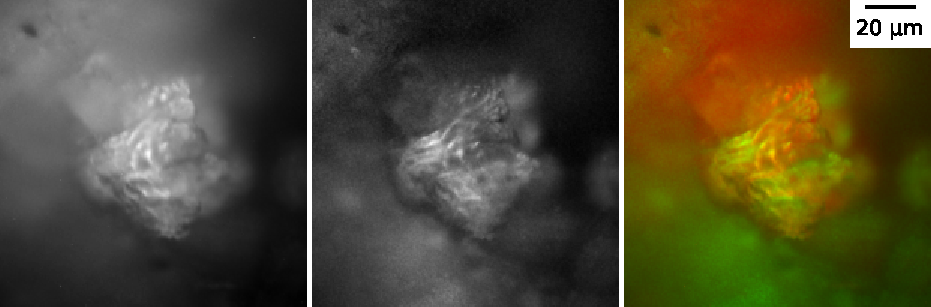
\includegraphics[width=\linewidth]{24508.pdf}
	\end{center}
	\vspace{-14mm}
	\begin{tabularx}{\textwidth}{XXX}
		\color{white}(a) & \color{white}(b) & \color{white}(c)
	\end{tabularx}
	\caption{Images of a mammal bone cortex. (a) Sum of all illumination directions includes both SHG and TPEF contributions. (b) SHG image separated from image (a). (c) Combined TPEF (red) and SHG (green) image. Intensity scales are different between images and color channels.}
	\label{fig:bone}
\end{figure}


\section{Conclusion}
In conclusion, we got fed up of using the word template and made this for all the interested people to use.

\section*{Acknowledgements}
We acknowledge the Flagship of Photonics Research and Innovation (PREIN) funded by the Academy of Finland (Grant No. 320165).

\begin{thebibliography}{99} %% use BibTeX or add references manually

\end{thebibliography}

\end{document}
